
\section{Application Acceleration}
\label{sec:acceleration}
\begin{figure}[t!]
	\centering
	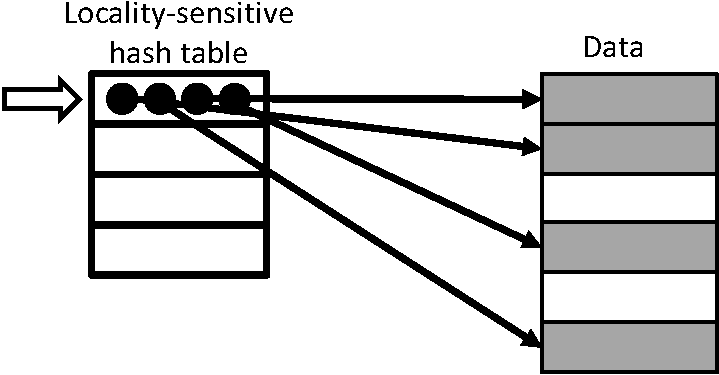
\includegraphics[width=0.25\textwidth]{figures/lsh-crop.pdf}
	\caption{Data accesses in LSH are randomly distributed}
	\label{fig:lsh}
\end{figure}


\begin{figure*}[t]
\centering
\vspace{0pt}
\begin{minipage}[t]{.2\textwidth}
	\includegraphics[width=0.2\paperwidth]{graphs/obj/hammingfull-crop.pdf}
	\caption{Nearest neighbor with BlueDBM up to two nodes}
	\label{fig:result_hammingfull}
\end{minipage}\hfill
\vspace{0pt}
\begin{minipage}[t]{.2\textwidth}
	\includegraphics[width=0.2\paperwidth]{graphs/obj/hammingdram-crop.pdf}
	\caption{Nearest neighbor with mostly DRAM}
	\label{fig:result_hammingdram}
\end{minipage}\hfill
\vspace{0pt}
\begin{minipage}[t]{.2\textwidth}
	\includegraphics[width=0.2\paperwidth]{graphs/obj/hammingsamsung-crop.pdf}
	\caption{Nearest neighbor with off-the-shelf SSD}
	\label{fig:result_hammingsamsung}
\end{minipage}\hfill
\vspace{0pt}
\begin{minipage}[t]{.2\textwidth}
	\includegraphics[width=0.2\paperwidth]{graphs/obj/hammingisp-crop.pdf}
	\caption{Nearest neighbor with in-store processing}
	\label{fig:result_hammingisp}
\end{minipage}
\end{figure*}

In this section, we demonstrate the performance and benefits of the BlueDBM
architecture by presenting some accelerator demonstrations. 

\subsection{Nearest Neighbor Search}


\paragraph{Description:}
Nearest neighbor search is required by many applications, e.g., image querying. One of
the modern techniques in this field is Locality Sensitive Hashing~\cite{lsh}.
LSH hashes the dataset using multiple hash functions, so that
similar data is statistically likely to be hashed to similar buckets. When
querying, the query is hashed using the same hash functions, and only the data
in the matching buckets are actually compared. The bulk of the work during a
query process is traversing hash buckets and reading the corresponding data to
perform distance calculation. Because data pointed to by the hash buckets are
most likely scattered across the dataset, access patterns are quite random (See Figure~\ref{fig:lsh}).




We have built a LSH query accelerator, where all of the data is stored in flash
and the distance calculation is done by the in-store processor on the storage
device. For simplicity, we assume 8KB data items, and calculate the hamming
distance between the query data and each of the items in the hash bucket. The
software sends a stream of addresses from a hash bucket along with the query
data page, and the system returns the index of the data item most closely matching the
query. Since we do not expect any performance difference for queries emanating from two different hash buckets, we simply send out a million nearest-neighbor searches for the same query.

\paragraph{Evaluation:}
In this study, we were interested in evaluating and comparing the benefits of
flash storage (as opposed to DRAM) and in-store processors.  We also wanted to
compare the BlueDBM design with off-the-shelf SSDs with PCIe interface. The
following experiments aims to evaluate the performance of each system during
various access patterns, such as random or sequential access, and when accesses
are partially serviced by secondary storage.

We have used a commercially available M.2 mPCIe SSD, whose performance, for 8KB
accesses, was limited to 600MB/s. Since BlueDBM performance is much higher
(2.4GB/s), we also conducted several experiments with BlueDBM throttled to
600MB/s. Since performance should scale linearly with the number of nodes for
this application, we concentrated on various configurations in a single node
setting:

\begin{enumerate}
\item Baseline: BlueDBM with in-store acceleration;
\item Baseline-T: Throttled BlueDBM with in-store acceleration;
\item H-DRAM: Multithread software on multi-core host accessing host DRAM as storage;
\item H-F Throttled: Multithreaded software on multi-core host accessing Throttled BlueDBM as storage;
\item DRAM + 10\% Flash: Same as H-DRAM with 10\% accesses to SSD; 
\item DRAM + 5\% Disk: Same as H-DRAM with 5\% accesses to HDD;
\item H-RFlash: Multithreaded software on multi-core host accessing
Off-the-shelf SSD;
\item H-SFlash: Same as H-RFlash except data accesses are artificially arranged to be sequential.
\end{enumerate}

Figure~\ref{fig:result_hammingfull} shows the relative performance of a
throttled BlueDBM (Baseline-T) and multithreaded software accessing data on
host DRAM (H-DRAM), with Baseline BlueDBM. The baseline performance we
observed on BlueDBM was 320K Hamming Comparisons per second. There are two
important takeaways from this graph. (1) BlueDBM can keep up with
DRAM-resident data for up to 4 threads, because host is getting compute-bound.
However, as more threads are added, performance will scale, until DRAM bandwidth
becomes the bottleneck. Since DRAM bandwidth as compared to flash bandwidth is
very high, DRAM-based processing wins with enough resources. (2) Native flash
speed matters i.e., when flash performance is throttled to 1/4th of the maximum, the performance drops accordingly. The relationship between flash performance and application performance will not be so simple if flash was being accessed by software.

To make the comparisons fair, we conducted a set of experiments shown in
Figures~\ref{fig:result_hammingdram},~\ref{fig:result_hammingsamsung},~\ref{fig:result_hammingisp} using throttled BlueDBM as the baseline. 

Results of DRAM + 5\% Disk and DRAM + 10\% Flash experiments shown in
Figure~\ref{fig:result_hammingdram} show that the performance of ram cloud (H-DRAM) falls off very sharply if even a small fraction of data does not reside in DRAM. Assuming 8 threads, the performance drops from 350K Hamming Comparisons per second to $<$ 80K and $<$ 10K Hamming Comparisons per second for DRAM + 10\% Flash and DRAM + 5\% Disk, respectively. At least one commercial vendor has observed similar phenomena and claimed that even when 40\% of data fits on DRAM, performance of Hadoop decreases by an order of magnitude~\cite{fusioniodram}. Complex queries on DRAM show high performance only as long as all the data fits in DRAM. 

The Off-the-shelf SSD experiment H-RFlash results in
Figure~\ref{fig:result_hammingsamsung} showed that its performance is poor as
compared to even throttled BlueDBM. However, when we artificially arranged the
data accesses to be sequential, the performance improved dramatically, sometimes
matching throttled BlueDBM. This suggests that the Off-the-shelf SSD may be optimized for sequential accesses.

Figure~\ref{fig:result_hammingisp} comparing Baseline-T and H-F Throttled shows the advantage of accelerators. In this example, the accelerator advantage is at least 20\%. Had we not throttled BlueDBM, the advantage would have been 30\% or more. This is because while the in-store processor can process data at full flash bandwidth, the software will be bottlenecked by the PCIe bandwidth at 1.6GB/s. We expect this advantage to be larger for applications requiring more complex accelerators
Compared to a fully flash-based execution, BlueDBM performs an order
of magnitude faster.

\subsection{Graph Traversal}

\paragraph{Description:}
Efficient graph traversal is a very important component of any graph processing
system. Fast graph traversal enables solving many problems in graph theory,
including maximum flow, shortest path and graph search. It is also a very
latency-bound problem because one often cannot predict the next node to visit,
until the previous node is visited and processed. We demonstrate the performance
benefits of our BlueDBM architecture by implementing distributed graph
traversal that takes advantages of the in-store processor and the integrated
storage network, which allows extremely low-latency access into both local and
remote flash storage.  

\paragraph{Evaluation:}
Graph traversal algorithms often involve dependent lookups. That is, the data from the first request determines the next request, like a linked-list traversal at the page level. Since such traversals are very sensitive to latency, we conducted the experiments with settings that are very similar to the settings in Section~\ref{sec:latency}.

\begin{enumerate}
\item IPS-F:  In-store processor requests data from remote storage over integrated network
\item H-F:  Software requests data from remote storage over integrated network 
\item H-RH-F:  Software requests data from remote software to read from flash
\item DRAM + 50\% F:  Store requests data from remote software. 50\% chance of hitting flash
\item DRAM + 30\% F:  Store requests data from remote software. 30\% chance of hitting flash
\item H-DRAM:  Software requests data from remote software. Data read from DRAM 
\end{enumerate}

As expected the results in Figure~\ref{fig:result_graph} show that the integrated storage network and in-store processor together show almost a factor of 3 performance improvement over generic distributed SSD. This performance difference is large enough that even when 50\% of the accesses can be accommodated by DRAM, performance of BlueDBM is still much higher.

The performance difference between \emph{H-F} and \emph{H-RH-F} illustrates the benefits of using the integrated network to reduce a layer of software access. Performance of \emph{ISP-F} compared to \emph{H-F} shows the benefits of further reducing software overhead by having the ISP manage the graph traversal logic. 
	
\begin{figure}[t]
	\centering
	\includegraphics[width=0.27\textwidth]{graphs/obj/graph-crop.pdf}
	\caption{Graph traversal performance}
	\label{fig:result_graph}
\end{figure}

%The difference latency has on graph traversal queries can
%be seen in Figure~\ref{fig:graph_accel}.
%\begin{figure}[ht!]
%	\centering
%
%		\hfill
%	\subfloat[Using ISP and Integrated Network]
%		{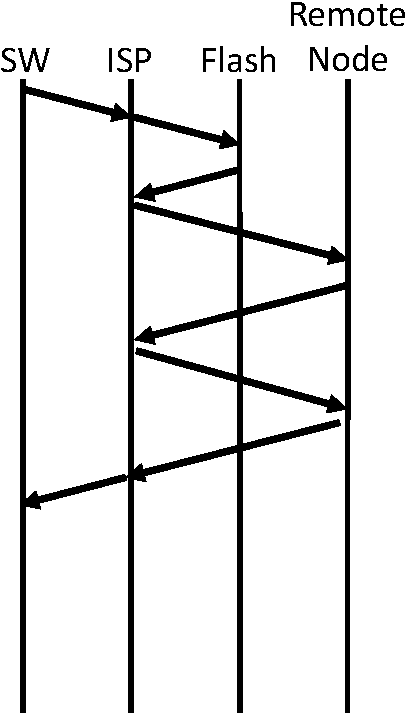
\includegraphics[width=0.12\textwidth]{figures/graph_isp-crop.pdf}}
%		\hfill
%	\subfloat[Using Software]
%		{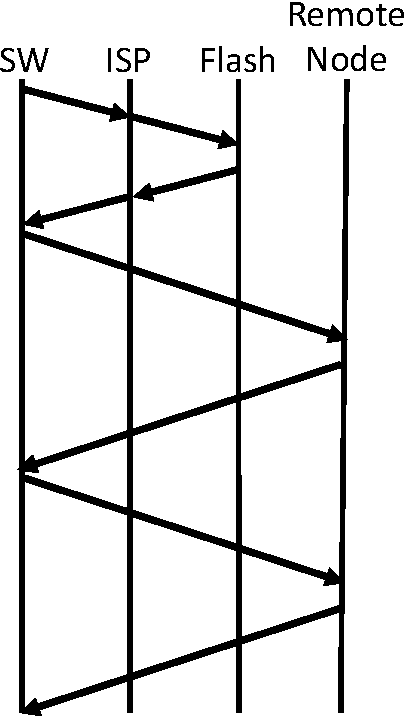
\includegraphics[width=0.12\textwidth]{figures/graph_sw-crop.pdf}}
%		\hfill
%	\caption{Graph Traversal Comparison}
%	\label{fig:graph_accel}
%\end{figure}

\subsection{String Search}

\paragraph{Description:}
String search is common operation in analytics, often used in
database table scans, DNA sequence matching and cheminformatics. It is 
primarily a sequential read and compare workload. We
examine its performance on BlueDBM with assistance from in-store Morris-Pratt (MP) 
string search engines~\cite{mpalgo} fully integrated with the file system, flash controller
and application software.  The software portion of string search initially sets
up the accelerator by transferring the target string pattern (needle) and a set
of precomputed MP constants over DMA. Then it consults the file system for a
list of physical addresses of the files to search (haystack).  This list is
streamed to the accelerator, which uses these addresses to request for pages
from the flash controller.  The accelerated MP engines may operate in parallel
either by searching multiple files or by dividing up the haystack into equal
segments (with some overlaps). This choice depends on the number of files and
size of each file. Since 4 read commands can saturate a single flash bus, we
use 4 engines per bus to maximize the flash bandwidth. Only
search results are returned to the server. 

\paragraph{Evaluation:}
We compared our implementation of hardware-accelerated string search running on
BlueDBM to the Linux Grep utility querying for exact string matches running
on both SSD and hard disk. Processing bandwidth and server CPU utilizations are
shown in Figure~\ref{fig:result_strstr}. We observe that the parallel MP
engines in BlueDBM are able to process a search at 1.1GB/s, which is 92\% of
the maximum sequential bandwidth a single flash board. Using BlueDBM, the
query consumes almost no CPU cycles on the host server since the query is
entirely offloaded and only the location of matched strings are returned, which
we assume is a tiny fraction of the file (0.01\% is used in our experiments).
This is 7.5x faster than software string search (Grep) on hard disks, which is
I/O bound by disk bandwidth and consumes 13\% CPU. On SSD, software string
search remains I/O bound by the storage device, but CPU utilization increases
significantly to 65\% even for this type of simple streaming compare operation.
This high utilization is problematic because string search is often only a small portion 
of more complex analytic queries that can quickly become compute bound.  As we
have shown in the results, BlueDBM can effectively alleviate this by
offloading search to the in-store processor thereby freeing up the server CPU
for other tasks. 
 


\begin{figure}[t]
	\centering
	\includegraphics[width=0.30\textwidth]{graphs/obj/strstr-crop.pdf}
	\caption{String search bandwidth and CPU utilization}
	\label{fig:result_strstr}
\end{figure}

